\section{Présentation d'Alter Solutions Engineering}
Alter Solutions Engineering, et plus particulièrement sa filiale Alter Frame, est l'entreprise qui m'a accueilli pour la durée de mon stage de fin d'études, nous allons donc commencer par la présenter rapidement.

\subsection{Les subdivisions d'Alter Solutions Engineering et leurs secteurs d'activité}
Alter Solutions Engineering est une entreprise relativement jeune : elle a été créée en 2006 et, si elle n'entre plus maintenant dans la catégorie des PME en termes de nombre de collaborateurs, elle reste une structure de petite taille.

Le siège social de l'entreprise se trouve à Versailles et c'est là où travaille l'équipe de développement française dont je fais partie. En pratique, il s'agit de l'équipe de développement d'Alter Frame qui est une entité enfant d'Alter Solutions Engineering (cf. section~\ref{subsec:frame}).

Alter Solutions Engineering est une société de conseil en hautes technologies mais en pratique, elle est composée de trois filières qui ont chacune une spécialité bien distinctes (cf. graphique~\ref{fig:filiales}).
\begin{figure}
  \centering
  \caption{Alter Solutions Engineering et ses filiales}
  \label{fig:filiales}
  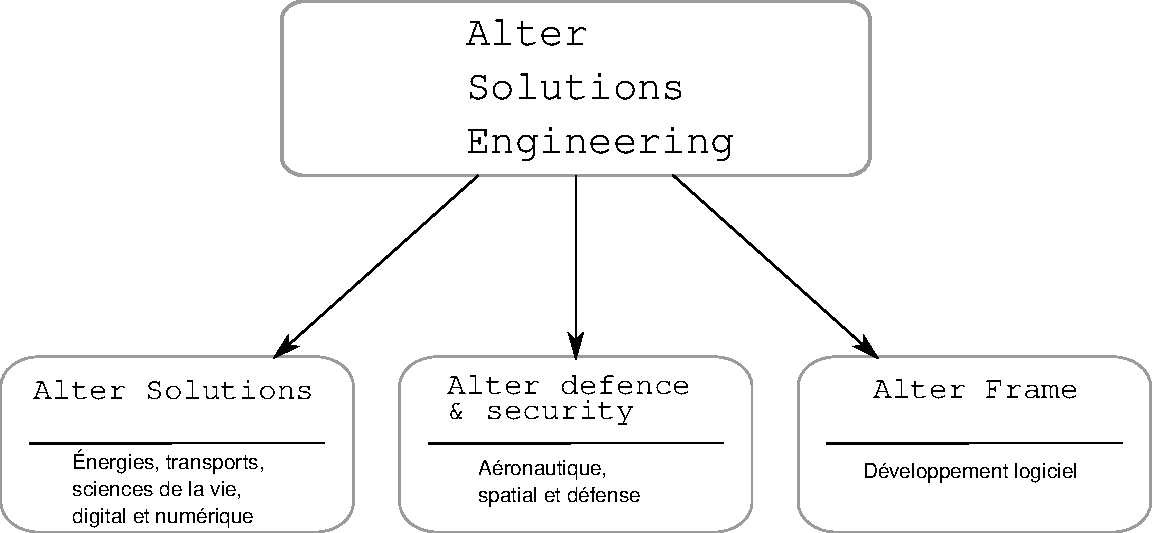
\includegraphics[width=\textwidth]{images/filiales_allinone.pdf}
\end{figure}

\subsubsection{Alter Solutions}
Cette filiale est spécialisée dans le conseil en ingénierie, notamment dans les domaines de l'énergie, des transports, des sciences de la vie, du digital et du numérique.

\subsubsection{Alter defence \& security}
Alter defence est également orientée vers le conseil, mais cette fois plus particulièrement dans l'aéronautique, le sptial et la défense.

Alter Defence and Security est également la filiale d'Alter Solutions Engineering qui m'accueillera une fois mon stage terminé (cf. section~\ref{sec:avenir}). L'objectif du groupe Alter au-travers de ce stage est de me donner le bagage technique et l'entraînement nécessaires pour pouvoir à terme me déployer comme expert technique auprès de clients de l'entreprise, or les missions de cyber-sécurité sont le domaine d'activité de Defence \& Security.

\subsubsection{Alter Frame}
Alter Frame enfin est la branche spécialisée dans l'édition de logiciels et celle que j'ai rejoint durant mon stage. C'est une ESN\footnote{Entreprise de Services du Numérique, cf. \url{https://fr.wikipedia.org/wiki/Entreprise_de_services_du_num\%C3\%A9rique}} dont l'activité est elle-même répartie en deux catégories :
\begin{itemize}[label=$\bullet$]
\item le conseil, c'est-à-dire le fait de fournir des spécialistes d'un domaine du numérique pour la durée d'un contrat à un client ;
\item le développement de logiciels au forfait, c'est-à-dire le fait de prendre commande d'un logiciel à réaliser en interne et de le livrer à la fin du contrat.
\end{itemize}

\subsection{Un peu plus de détails sur Alter Frame}
\label{subsec:frame}
Bien qu'Alter Frame ait des clients et des domaines d'intervention variés, en termes de technologes il y a trois pôles de compétences qui sont caractéristiques de l'entreprise et reviennent le plus régulièrement :
\begin{itemize}[label=$\bullet$]
\item Java ;
\item .NET ;
\item PHP.
\end{itemize}

Mon stage ne s'est pas cantonné au domaine du développement mais il en a tout de même inclus celui-ci s'est déroulé au sein de l'équipe Java.

\subsection{Quelques (derniers) chiffres}
TODO : À remettre en forme pour plus tard
Mettre une note\footnote{\url{http://www.alter-solutions.com/notre-societe/chiffres-cles/}}.
375 collaborateurs en France, Portugal et Belgique (combien dans chaque pays ?)

\subsection{Répartition de l'activité}
\begin{tikzpicture}
    \pie[color ={orange!100, orange!80, orange!60,  orange!40, orange!20, orange!10}, explode=0.1]{33/Énergies, 20/Aéronautique spatial et défense, 18/Transports, 11/Dgital et numérique, 10/Industrie, 8/Sciences de la vie}
\end{tikzpicture}
test